% !TEX encoding = UTF-8 Unicode
%%%%%%%%%%%%%%%%%%%%%%%%%%%%%%%%%%%%%%%%%%%%%%%%%%%%%%%%%%%%%%%%%%%%%%%%%%%%%%%%
%% Tikzposter is highly customizable: please see                              %%
%% https://bitbucket.org/surmann/tikzposter/downloads/styleguide.pdf          %%
%%%%%%%%%%%%%%%%%%%%%%%%%%%%%%%%%%%%%%%%%%%%%%%%%%%%%%%%%%%%%%%%%%%%%%%%%%%%%%%%

\documentclass[17pt,a1paper,portrait]{tikzposter}

%//////////////////////////////////////////////////////////////////////////////%
%------------------------------------------------------------------------------%
%                                 CONFIGURATION                                %
%------------------------------------------------------------------------------%
%\\\\\\\\\\\\\\\\\\\\\\\\\\\\\\\\\\\\\\\\\\\\\\\\\\\\\\\\\\\\\\\\\\\\\\\\\\\\\\%

%==============================================================================%
%                                     THEME                                    %
%==============================================================================%

%%%%%%%%%%%%%%%%%%%%%%%%%%%%%%%%%%%%%%%%%%%%%%%%%%%%%%%%%%%%%%%%%%%%%%%%%%%%%%%%
%% Available themes: see also                                                 %%
%% https://bitbucket.org/surmann/tikzposter/downloads/themes.pdf              %%
%%%%%%%%%%%%%%%%%%%%%%%%%%%%%%%%%%%%%%%%%%%%%%%%%%%%%%%%%%%%%%%%%%%%%%%%%%%%%%%%

% \usetheme{Default}
% \usetheme{Rays}
% \usetheme{Basic}
% \usetheme{Simple}
% \usetheme{Envelope}
% \usetheme{Wave}
% \usetheme{Board}
\usetheme{Autumn}
% \usetheme{Desert}

% \usecolorstyle [colorPalette=GreenGrayViolet]{Default}
\useinnerblockstyle{Table}

%==============================================================================%
%                                     COLORS                                   %
%==============================================================================%

% Power point colors
\definecolor{ms-purple}{HTML}{403152}
\definecolor{ms-blue}{HTML}{254061}
\definecolor{ms-red}{HTML}{98071B}
\definecolor{ms-green}{HTML}{4F6228}
\definecolor{ms-cyan}{HTML}{215968}
\definecolor{ms-brown}{HTML}{632523}
\definecolor{citation}{HTML}{FAFAFA}

\definecolorstyle{myColorStyle}{
  \colorlet{colorOne}{ms-red}
  \colorlet{colorTwo}{gray}
%   \colorlet{colorThree}{mygray}
}{
  % Background Colors
  \colorlet{backgroundcolor}{colorTwo!2}
%   \colorlet{framecolor}{colorTwo!50}
  % Title Colors
%   \colorlet{titlefgcolor}{white}
  \colorlet{titlebgcolor}{colorOne}
  % Block Colors
  \colorlet{blocktitlebgcolor}{colorOne}
  \colorlet{blocktitlefgcolor}{white}
%   \colorlet{blockbodybgcolor}{colorTwo!50}
%   \colorlet{blockbodyfgcolor}{black}
  % Innerblock Colors
  \colorlet{innerblocktitlebgcolor}{colorOne}
  \colorlet{innerblocktitlefgcolor}{white}
  \colorlet{innerblockbodybgcolor}{white}
  \colorlet{innerblockbodyfgcolor}{black}
  % Note colors
%   \colorlet{notefgcolor}{black}
%   \colorlet{notebgcolor}{white}
%   \colorlet{notefrcolor}{white}
}
\usecolorstyle{myColorStyle}


%==============================================================================%
%                                     COLORS                                   %
%==============================================================================%

% Power point colors

\definecolor{my-black}{HTML}{594F4F}
\definecolor{my-darkblue}{HTML}{547980}
\definecolor{my-blue}{HTML}{45ADA8}
\definecolor{my-green}{HTML}{9DE0AD}
\definecolor{my-lightgreen}{HTML}{E5FCC2}


\definecolorstyle{myColorStyle}{
  \colorlet{colorOne}{my-darkblue}
  \colorlet{colorTwo}{my-black}
}{
  % Background Colors
  \colorlet{backgroundcolor}{colorTwo!2}
  % Title Colors
  \colorlet{titlebgcolor}{colorOne}
  % Block Colors
  \colorlet{blocktitlebgcolor}{colorOne}
  \colorlet{blocktitlefgcolor}{white}
  % Innerblock Colors
  \colorlet{innerblocktitlebgcolor}{colorOne}
  \colorlet{innerblocktitlefgcolor}{white}
  \colorlet{innerblockbodybgcolor}{white}
  \colorlet{innerblockbodyfgcolor}{black}
  % Note colors
%   \colorlet{notefgcolor}{black}
%   \colorlet{notebgcolor}{white}
%   \colorlet{notefrcolor}{white}
}
\usecolorstyle{myColorStyle}

%==============================================================================%
%                                     BLOCKS                                   %
%==============================================================================%

\defineblockstyle{myBlockStyle}{
  titlewidthscale=1.0, bodywidthscale=1,titleleft,
  titleoffsetx=0pt, titleoffsety=0pt, bodyoffsetx=0mm, bodyoffsety=0mm,
  bodyverticalshift=0mm, roundedcorners=5, linewidth=2pt,
  titleinnersep=6mm, bodyinnersep=10mm
}{
\draw[color=framecolor, fill=blockbodybgcolor,
  rounded corners=\blockroundedcorners] (blockbody.south west)
  rectangle (blockbody.north east);
  \ifBlockHasTitle
    \draw[color=framecolor, fill=blocktitlebgcolor,
    rounded corners=\blockroundedcorners] (blocktitle.south west)
    rectangle (blocktitle.north east);
  \fi
}
\useblockstyle{myBlockStyle}

\defineinnerblockstyle{myInnerblockStyle}{
  titlewidthscale=1.0, bodywidthscale=1,titlecenter,
  titleoffsetx=0pt, titleoffsety=0pt, bodyoffsetx=0mm, bodyoffsety=0mm,
  bodyverticalshift=0mm, roundedcorners=5, linewidth=4pt,
  titleinnersep=4mm, bodyinnersep=5mm
}{
\draw[color=framecolor, fill=innerblockbodybgcolor,
  rounded corners=\innerblockroundedcorners] (innerblockbody.south west)
  rectangle (innerblockbody.north east);
  \ifInnerblockHasTitle
    \draw[color=framecolor, fill=innerblocktitlebgcolor,
    rounded corners=\innerblockroundedcorners] (innerblocktitle.south west)
    rectangle (innerblocktitle.north east);
  \fi
}
\useinnerblockstyle{myInnerblockStyle}

%//////////////////////////////////////////////////////////////////////////////%
%------------------------------------------------------------------------------%
%                                    PREAMBLE                                  %
%------------------------------------------------------------------------------%
%\\\\\\\\\\\\\\\\\\\\\\\\\\\\\\\\\\\\\\\\\\\\\\\\\\\\\\\\\\\\\\\\\\\\\\\\\\\\\\%

%==============================================================================%
%                                    PACKAGES                                  %
%==============================================================================%

% Language
\usepackage[brazil]{babel}
\usepackage[T1]{fontenc}
\usepackage[utf8]{inputenc}
\usepackage{amsfonts}
\usepackage{amssymb}
\usepackage{mathtools}  
% Encoding

% References
\usepackage{hyperref}
\hypersetup{
  colorlinks  = true, %Colours links instead of ugly boxes
  urlcolor    = ms-red, %Colour for external hyperlinks
  linkcolor   = ms-purple, %Colour of internal links
  citecolor   = ms-purple, %Colour of citations
}

% Font theme
\usepackage[default]{droidserif}
\usepackage[defaultsans]{droidsans}

% Positions
\usepackage{caption}
\usepackage{adjustbox}

% Authblk
\usepackage{authblk}
\renewcommand\Authand{ e }
\renewcommand\Authands{, e }
\renewcommand\Authfont{\LARGE}
\renewcommand\Affilfont{\normalsize}

% Bibliography
\usepackage{csquotes}
\usepackage[backend=bibtex]{biblatex}


\bibliography{post}
%//////////////////////////////////////////////////////////////////////////////%
%------------------------------------------------------------------------------%
%                                    DETAILS                                   %
%------------------------------------------------------------------------------%
%\\\\\\\\\\\\\\\\\\\\\\\\\\\\\\\\\\\\\\\\\\\\\\\\\\\\\\\\\\\\\\\\\\\\\\\\\\\\\\%

%==============================================================================%
%                                      INFO                                    %
%==============================================================================%

\graphicspath{{./figuras/}}

\title{\parbox{\linewidth}{\centering
  \vspace{-1em}
  Implementação de algoritmo de consulta de segmentos em janelas
  \bigskip\bigskip
}}

\author{Aluno: Mateus Barros Rodrigues\\Orientador: Prof. Dr. Carlos Eduardo Ferreira}
\affil{
  Instituto de Matemática e Estatística - Universidade de São Paulo\\%
  \texttt{mateus.barros.rodrigues@ime.usp.br}%
  \vspace{-3em}
}

% Avoid shifting of blocks
\makeatletter
\def\maketitle{\AB@maketitle}
\makeatother

%==============================================================================%
%                                  BIBLIOGRAPHY                                %
%==============================================================================%

\renewcommand*{\bibfont}{\scriptsize}

%==============================================================================%
%                                    CAPTION                                   %
%==============================================================================%

\DeclareCaptionType{diagram}[Diagrama][Lista de diagramas]

%//////////////////////////////////////////////////////////////////////////////%
%------------------------------------------------------------------------------%
%                                    CONTENT                                   %
%------------------------------------------------------------------------------%
%\\\\\\\\\\\\\\\\\\\\\\\\\\\\\\\\\\\\\\\\\\\\\\\\\\\\\\\\\\\\\\\\\\\\\\\\\\\\\\%

\begin{document}
\maketitle

%##############################################################################%

\begin{columns}

%==============================================================================%

\column{0.30}

%------------------------------------------------------------------------------%

{\colorlet{blocktitlebgcolor}{my-blue}\block{Introdução}{ Este trabalho de conclusão de curso fundamentou-se na compreensão e
    implementação (em linguagem \emph{python}) de um algoritmo para consultas de intersecções de segmentos de retas com janelas
    retangulares no espaço. Este é  um problema de geometria computacional conhecido por: buscas em regiões ortogonais. Este algoritmo
    foi o foco da tese de mestrado de Álvaro Junio Pereira Franco \cite{junio09:MSc}. Além da implementação, foi feita também a
    adaptação do visualizador de algoritmos geométricos feito por Alexis Sakurai Landgraf para exposição dos resultados obtidos.
}}

%------------------------------------------------------------------------------%

{\colorlet{blocktitlebgcolor}{my-green}\block{Consultas em janelas}{ Neste trabalho foi abordado o problema de \emph{consultas de
      segmentos em janelas}, um problema de buscas em intervalos ortogonais. Dado um conjunto $S$ de segmentos não-intersectantes
    no espaço (seja em $\mathbb{R}$ ou $\mathbb{R}^2$) queremos organizar os segmentos em estruturas de dados para que possamos
    responder eficientemente consultas do tipo: \emph{dada uma janela $W$ de lados paralelos, quais segmentos de S estão contidos
      ou intersectam a janela W?}\\

    Para resolvermos esse problema eficientemente, começamos criando 4 estruturas baseadas em $S$: duas \textbf{árvores limite com
      camadas}, uma sobre o conjunto de pontos esquerdos de $S$ e outra sobre o conjunto de pontos direitos de $S$, e duas
    \textbf{árvores de segmentos 2D}, uma horizontal e a outra vertical.\\

    Feito esse pré-processamento, a resposta da consulta será dividida em 5 etapas:\\

    \begin{itemize}
    \item[1.] Encontramos todos os segmentos com o ponto esquerdo dentro da janela. 
    \item[2.] Encontramos todos os segmentos com o ponto direito dentro da janela. 
    \item[3.] Encontramos todos os segmentos que intersectam com o lado esquerdo da janela.
    \item[4.] Encontramos todos os segmentos que intersectam com o lado direito da janela.
    \item[5.] Encontramos todos os segmentos que intersectam com o lado superior da janela.\\
    \end{itemize}
    
    Perceba que poderão haver segmentos que serão detectados em mais de uma dessas consultas, teremos então que remover as
    repetições na resposta final.

}}


  

%==============================================================================%

\column{0.35}

{\colorlet{blocktitlebgcolor}{my-green}\block{Simulação}{ Para exemplificarmos o tipo de problema resolvido, segue uma série
    de imagens tiradas do visualizador geométrico na resolução de uma consulta de segmentos:


    \begin{tikzfigure}
      \centering 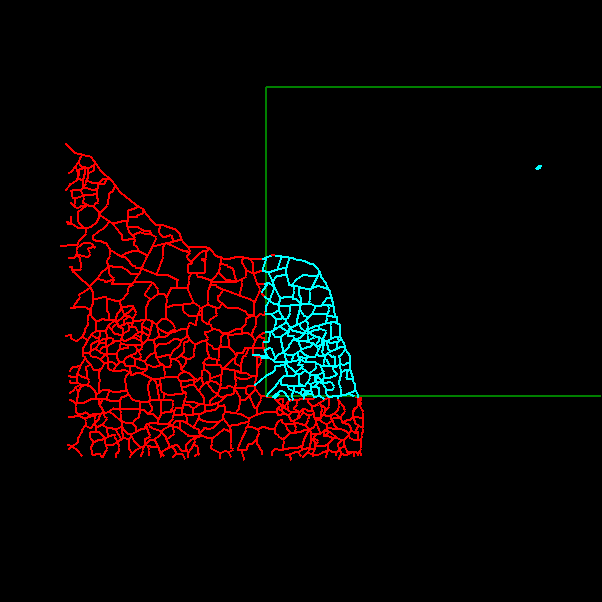
\includegraphics[width=0.9\linewidth]{2}
      \captionof{figure}{Destacamos em azul os segmentos cuja ponta esquerda
        está na janela e em amarelo os segmentos cuja ponta direita está na janela.}
      \label{diag:2}
    \end{tikzfigure}

    \begin{tikzfigure}
      \centering
      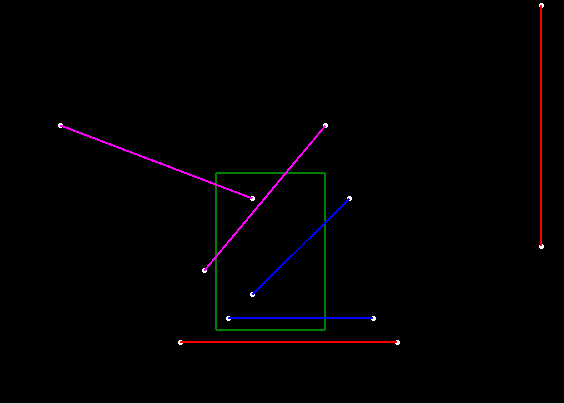
\includegraphics[width=0.9\linewidth]{3}
      %\captionsetup{type=diagram}
      \captionof{figure}{Destacamos em rosa os segmentos que intersectam com o lado esquerdo da janela.}
      \label{diag:3}
    \end{tikzfigure}

    \begin{tikzfigure}
      \centering
      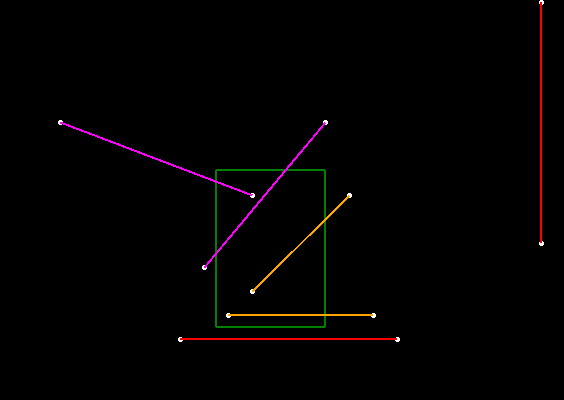
\includegraphics[width=0.9\linewidth]{4}
      %\captionsetup{type=diagram}
      \captionof{figure}{Destacamos em laranja os segmentos que intersectam com o lado direito da janela.}
      \label{diag:4}
    \end{tikzfigure}

    \begin{tikzfigure}
      \centering
      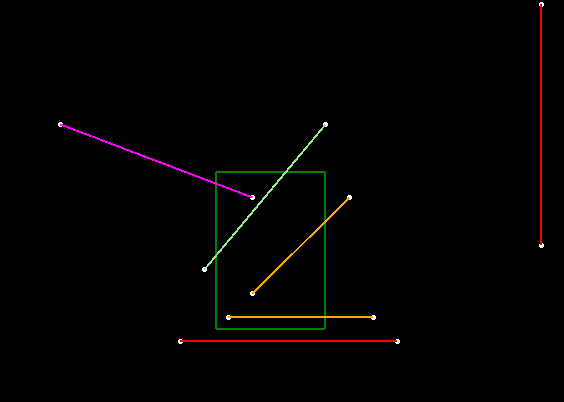
\includegraphics[width=0.9\linewidth]{5}
      %\captionsetup{type=diagram}
      \captionof{figure}{Destacamos em verde-claro os segmentos que intersecam com o lado superior da janela.}
      \label{diag:5}
    \end{tikzfigure}

}}

\column{0.35}

{\colorlet{blocktitlebgcolor}{my-green}\block{}{

    \begin{tikzfigure}
      \centering
      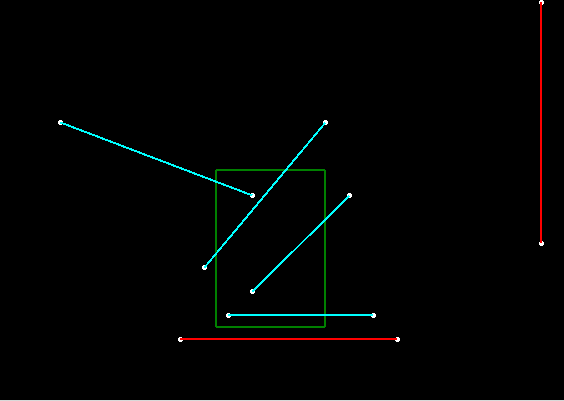
\includegraphics[width=0.9\linewidth]{6}
      %\captionsetup{type=diagram}
      \captionof{figure}{Destacamos em azul-claro todos os segmentos contidos na janela dada.}
      \label{diag:6}
    \end{tikzfigure}
}}

{\colorlet{blocktitlebgcolor}{my-darkblue}\block{Mais exemplos}{
    \begin{tikzfigure}
      \centering
      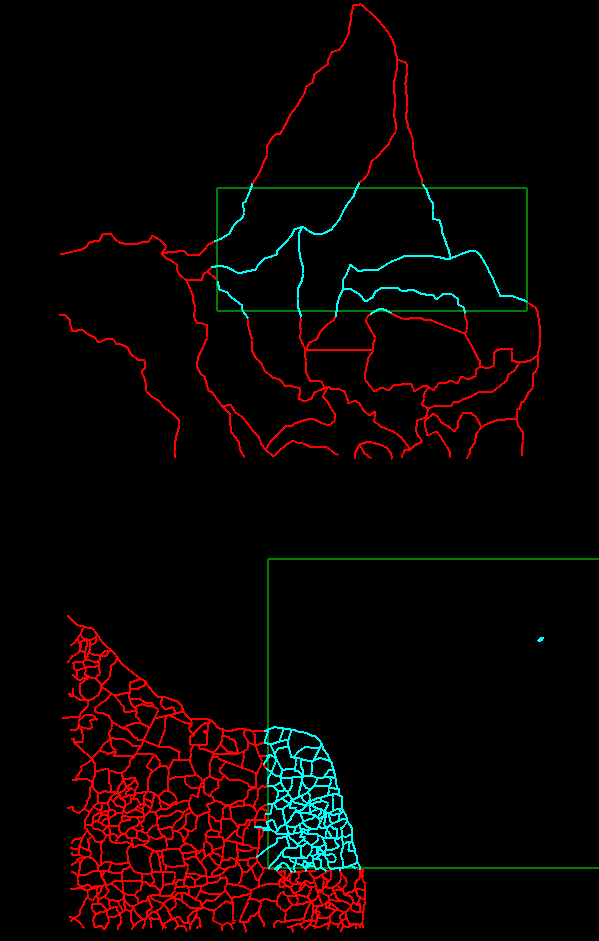
\includegraphics[width=0.9\linewidth]{7}
      %\captionsetup{type=diagram}
      \captionof{figure}{Dois exemplos de janelas em partes de um mapa de municípios do Brasil.}
      \label{diag:7}
    \end{tikzfigure}

}}


{\colorlet{blocktitlebgcolor}{my-blue}\block{Conclusão}{ Todos os algoritmos, sejam os utilizados efetivamente na consulta que nos
    propomos a resolver ou os mais básicos utilizados para fins de estudo, foram descritos de forma didática no trabalho, contando
    com sua implementação em linguagem \emph{python} (disponível também no gitHub~\cite{site}) e análise de complexidade
    correspondente.  }}

{\colorlet{blocktitlebgcolor}{my-black}\block{Referências}{
    \inputencoding{latin2}
    \printbibliography[heading=none]
}}

%------------------------------------------------------------------------------%
%==============================================================================%

\end{columns}

%##############################################################################%

\end{document}

